\chapter{Dynamic Model of the Quadrotor \label{ch:model}}

In this chapter, the dynamics of the quadrotor and the calculation of the mathematical model through two different approaches, are provided. In addition, the necessary considerations for the choice of a geometry configuration are exposed. This dynamic model and its inputs setting are needed to design the quadrotor flight controllers.
\\\\
Section \ref{sec:configurations} presents the description of two of the main used quadrotor geometry configurations. Also, this section presents what it means to choose one or the other configuration for the setting of the quadrotor inputs.
\\\\
The dynamic model of the quadrotor, obtained using the Newton-Euler and Euler-Lagrange approaches, neglecting the gyroscopic effects produced by the propellers, is shown in Section \ref{sec:nonlinear}.
\\\\
Finally, Section \ref{sec:linearized} describes an overview of the Jacobian linearization method applied to the quadrotor dynamic model and the thrust compensation needed to be implemented in a real quadrotor.

\section{Quadrotors Configurations}
\label{sec:configurations}
The term `quadrotor' refers to a rotary-wing UAV which thrust is generated using four motors and propellers. Quadrotors can be build in multiple ways.
There are two basic configurations which are widely used by commercial manufacturers and hobbyists. These two configurations are the `+' and the `X'.
%\\\\
%\url{https://www.google.com/search?q=why+\%2B+or+x+configuration+quadcopter&ie=utf-8&oe=utf-8&client=firefox-b-ab&gfe_rd=cr&dcr=0&ei=Mr0BWrW9HtHk8AfXm7fADQ}
%\\\\
%\url{https://community.micro-motor-warehouse.com/t/vs-x-configuration/2673}
%\\\\
%\url{https://www.quora.com/Why-is-x-configuration-preferred-over-+-config-of-quadcopter}
%\\\\
%\url{https://www.rcgroups.com/forums/showthread.php?1203569-Quad-X-vs-configuration}


\subsection{The `+' Configuration}
The geometry used in quadrotors built in `+' configuration is shown in Fig. \ref{fig:quadcopterplus}.
\\
\begin{figure}[H]
\begin{center}
  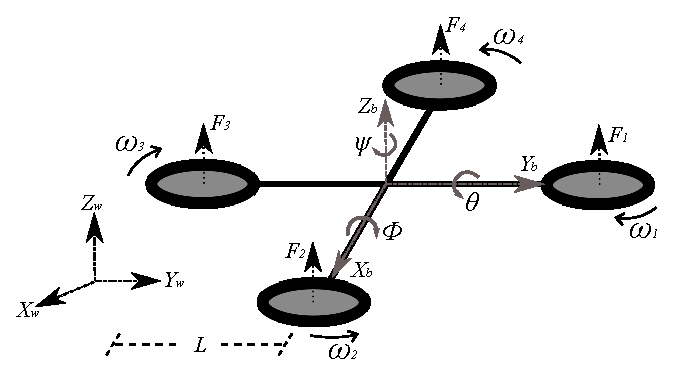
\includegraphics[width=0.90\textwidth]{quadcopterplus.eps}
\caption{Quadrotor geometry in `+' configuration} 
    \label{fig:quadcopterplus}
    \end{center}
\end{figure}
In Fig. \ref{fig:quadcopterplus}, ($\phi$, $\theta$, $\psi$) are the angular deviations (pitch, roll and yaw, respectively) of the quadrotor about the body-frame;
 ($x$, $y$, $z$) are the body-frame axes;  ($X_W$, $Y_W$, $Z_W$) are the earth-frame axes; $L$ is the distance from the quadrotor center of gravity ($CoG$) to the motors center; $F_{M_i}$ is the thrust force exerted by each motor $M_i$; and $\omega_i$ is the angular velocity of $M_i$, with $i = 1,2,3,4$. In this configuration, the body-frame axes $x$ and $y$, coincide with the lines that connect motors of opposite sides in the quadrotor frame.
\\\\
The quadrotor is a system with six $DoF$. Since a quadrotor has four actuators, it can be considered an underactuated system. This means that, it is only possible to reach a desired state for four $DoF$. However, it is possible to indirectly control the two remaining $DoF$ choosing the control signals appropriately. These control signals, or inputs, represent the quadrotor basic movements and are described below.

\begin{itemize}
\item \textbf{Thrust $T_u$ [$N$]}\\\\
The thrust $T_u$ is the total thrust force exerted parallel to the body-frame $z$-axis by the four motors. This thrust, can also generate accelerations in the direction of the $X_W$ and $Y_W$ axes. This happens when $|\theta| > 0$ or $|\phi| > 0$.
\\\\
This control signal affects the speed of rotation of all motors, and therefore their thrust, in equal magnitude, and is set as
\begin{equation}
\label{ec:u+}
T_u = \sum_{i=1}^{4}F_{M_i}.
\end{equation}

\item \textbf{Yaw Torque $\tau_{\psi}$ [$N\cdot m$]}\\\\
From Fig. \ref{fig:quadcopterplus}, $M_1$ and $M_3$ have a clockwise ($CW$) rotation while $M_2$ and $M_4$ rotate counter-clockwise ($CCW$). This configuration of opposite pairs rotational directions allows the system to control its conservation of momentum, and thus change its yaw angle in a controlled manner. This is done unbalancing the total momentum around the $z$-axis and without the need of a tail rotor used in the standard helicopter structure (\cite{Bresciani2008}). In `+' configuration, the fact that the pitch and roll angles are controlled using only two motors that rotate in the same direction, leads to large changes in the thrust force of the other two motors to achieve conservation of momentum.
\\\\
This conservation of momentum is controlled using the torque generated by each motor ($\tau_{M_i}$) around the body-frame $z$-axis. It produces a turn in the opposite direction to the rotation of the motor. Taking into account that the torque $\tau_\psi$ is positive when it generates a clock-wise rotation around the $z$-axis, only $M_2$ and $M_4$ contribute positively to it. While the other tow motors have a negative contribution to $\tau_\psi$. Thus, the total torque around the $z$-axis is depicted as
\begin{equation}
\label{ec:taupsiTM}
\tau_{\psi} = \tau_{M_2} + \tau_{M_4} - \tau_{M_1} - \tau_{M_3}.
\end{equation}
Each torque $\tau_{M_i}$ has a linear relationship with the thrust applied by the motor, with $K_M$ being the proportional constant and
\begin{equation}
\label{ec:taumi}
\tau_{M_{i}} = K_{M}F_{M_i}.
\end{equation}
Replacing (\ref{ec:taumi}) in (\ref{ec:taupsiTM}) the total torque $\tau_\psi$ dependence on the forces $F_{M_i}$ is got as
\begin{equation}
\label{ec:taupsi+}
\tau_{\psi} = K_{m}(F_{M_2} + F_{M_4} - F_{M_1} - F_{M_3}).
\end{equation}

\item \textbf{Roll Torque $\tau_{\theta}$ [$N\cdot m$]}\\\\
The roll torque $\tau_\theta$ is described as the torque exerted on the $x$-axis and about the $y$-axis. In the `+' configuration, the only motors that affect the quadrotor rotation with respect to the $x$-axis are $M_2$ and $M_4$. These do not affect the rotation with respect to the $y$-axis. In this case, the torques are generated by the forces $F_{M_2}$ and $F_{M_4}$ being applied at a distance $L$ from the quadrotor $CoG$. Considering a positive $\tau_\theta$ as the one causing a counter clock-wise rotation about the $y$-axis, the roll torque in `+' is set as
\begin{equation}
\label{ec:tautheta+}
\tau_{\theta} = L(F_{M_4}-F_{M_2}).
\end{equation}

\item \textbf{Pitch Torque $\tau_{\phi}$ [$N\cdot m$]}\\\\
Unlike the roll torque, the pitch torque $\tau_\phi$ is the one exerted on the $y$-axis about the $x$-axis. As Fig. \ref{fig:quadcopterplus} shows, $M_1$ and $M_3$ are the motors applying the forces that create this torque. Being $\tau_\phi$ positive when clock-wise rotation about the $x$-axis is caused, it is defined for a `+' configuration as
\begin{equation}
\label{ec:tauphi+}
\tau_{\phi} = L(F_{M_3}-F_{M_1}).
\end{equation}
\end{itemize}

\subsubsection{Inputs Setting in `+' Configuration}
Summarizing, the `+' configuration quadrotor inputs are established as linear combinations of the motors forces $F_{M_i}$. Equations (\ref{ec:u+}), (\ref{ec:taupsi+}), (\ref{ec:tautheta+}) and (\ref{ec:tauphi+}) integrate a linear equations system where the vector of inputs $\mathbf{u_{(+)}}$ is
\begin{equation}
	\mathbf{u_{(+)}} = \begin{bmatrix}
	T_u\\[5pt]
	\tau_{\psi}\\[5pt]
	\tau_{\theta}\\[5pt]
	\tau_{\phi}
	\end{bmatrix} = \begin{bmatrix}
	1 & 1 & 1 & 1 \\[5pt]
	-K_{m} & K_{m} & -K_{m} & K_{m}\\[5pt]
	0 & -L & 0 & L\\[5pt]
	-L & 0 & L & 0
							\end{bmatrix}
\begin{bmatrix}
F_{M_1}\\[5pt]
F_{M_2}\\[5pt]
F_{M_3}\\[5pt]
F_{M_4}
\end{bmatrix}.
	\label{ec:U_+}						
\end{equation}

\subsection{The `X' Configuration}
Following the same nomenclature used in the `+' configuration, in `X' configuration, the quadrotor frame is rotated $\pi/4\ rad$ about the $z$-axis in the body-frame, as shown in Fig. \ref{fig:quadrotorX}. 
\\\\
In this case, the front-line in the quadrotor is set between $M_1$ and $M_4$. In `X' configuration, the roll and pitch torques are applied using the forces exerted by all the motors at a distance $L_X = L\cdot \cos(\pi/4)$ (\cite{Faessler2016}).  This geometry is shown in Fig. \ref{fig:quadrotorX}.
\begin{figure}[H]
\begin{center}
  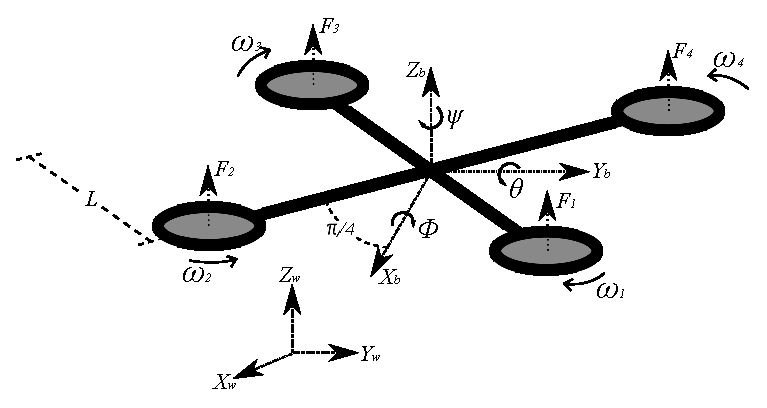
\includegraphics[width=0.97\textwidth]{quadcopter1.eps}
% figure caption is below the figure
\caption{Quadrotor geometry in `X' configuration} 
    \label{fig:quadrotorX}
    \end{center}
\end{figure}
The inputs description for the quadrotor `X' configuration is defined as follows.
\begin{itemize}
\item \textbf{Thrust $T_u$ [$N$]}\\\\
The total thrust exerted by the four motors in the quadrotor is not changed between the `+' and `X' configurations. Hence, the thrust $T_u$ is defined as
\begin{equation}
\label{ec:ux}
T_u = \sum_{i=1}^{4}F_{M_i}.
\end{equation}

\item \textbf{Yaw Torque $\tau_{\psi}$ [$N\cdot m$]}\\\\
As the $z$-axis is not modified between the `+' and `X' configurations, and the motors rotate in the same direction as in the other configuration, the yaw torque $\tau_\psi$ is set as
\begin{equation}
\label{ec:taupsix}
\tau_{\psi} = K_{m}(F_{M_2} + F_{M_4} - F_{M_1} - F_{M_3}).
\end{equation}
\\\\
\item \textbf{Roll Torque $\tau_{\theta}$ [$N\cdot m$]}\\\\
As shown in Fig. \ref{fig:quadrotorX}, roll and pitch torques are affected by the effects of all the quadrotor motors. For the roll torque $\tau_{\theta}$, the motors $M_3$ and $M_4$ contribute positively, while $M_1$ and $M_2$ have a negative contribution to it. In this case, the roll torque is depicted as
\begin{equation}
\label{ec:tauthetax}
\tau_{\theta} = L_{X}(F_{M_3}+F_{M_4}-F_{M_2}-F_{M_1}).
\end{equation}

\item \textbf{Pitch Torque $\tau_{\phi}$ [$N\cdot m$]}\\\\
Due to the $CW$ positive direction of the $\phi$ angle, and considering the sign of the contribution exerted by each force $F_{M_i}$, the pitch torque for the `X' configuration is defined as
\begin{equation}
\label{ec:tauphix}
\tau_{\phi} = L_{X}(F_{M_2}+F_{M_3}-F_{M_1}-F_{M_4}).
\end{equation}

\end{itemize}

\subsubsection{Inputs Setting in `X' Configuration}
In the `X' configuration, the quadrotor inputs remain the same regarding the `+' configuration. However both $\tau_\theta$ and $\tau_\phi$ are affected by the interaction of all the motors and the change in the distance of the point of application of the forces $F_{M_i}$ on the $x$ and $y$ axes. The linear equations system that shows the inputs setting for a quadrotor in `X' configuration is defined as
\begin{equation}
	\mathbf{u_{(X)}} = \begin{bmatrix}
	T_u\\[5pt]
	\tau_{\psi}\\[5pt]
	\tau_{\theta}\\[5pt]
	\tau_{\phi}
	\end{bmatrix} = \begin{bmatrix}
	1 & 1 & 1 & 1 \\[5pt]
	-K_{m} & K_{m} & -K_{m} & K_{m}\\[5pt]
	-L_{X} & -L_{X} & L_{X} & L_{X}\\[5pt]
	-L_{X} & L_{X} & L_{X} & -L_{X}
							\end{bmatrix}
\begin{bmatrix}
F_{M_1}\\[5pt]
F_{M_2}\\[5pt]
F_{M_3}\\[5pt]
F_{M_4}
\end{bmatrix}.
	\label{ec:U_X}						
\end{equation}

\subsubsection{Maximum Torque About $x$ and $y$ axes in `X' Configuration}
In `+' configuration, the torques around the $x$ and $y$ axes are set using just two motors applying a force at a distance $L$ from the quadrotor $CoG$. This implies that, for instance, in the case of roll torque $\tau_\theta$ the maximum torque $\tau_{\theta max (+)}$ is achieved when $F_{M_4} = F_{M_i max}$ and $F_{M_3} = 0$, where $F_{M_i max}$ is the maximum thrust of the motors. Then, in `+' configuration, the $\tau_{\theta max (+)}$ is set as
\begin{equation}
\tau_{\theta max (+)} = L\cdot F_{M_i max}
\end{equation}
On the other hand, the torques around the $x$ and $y$ axes in `X' configuration depend on the forces of the four motors in the quadrotor, which are applied at a distance $L_{X} = L\cdot \cos(\pi/4)$ from the quadrotor $CoG$. Continuing with the example of the roll torque, in `X' configuration the maximum torque $\tau_{\theta max (X)}$ is achieved when $F_{M_3} = F_{M_4} = F_{M_i max}$ and $F_{M_1} = F_{M_2} = 0$. Hence, the maximum torque about the $y$-axis in `X' configuration is
\begin{align}
\begin{split}
\tau_{\theta max (X)} & = L\cdot \cos(\pi/4) \cdot 2 \cdot F_{M_i max}\\[5px]
\tau_{\theta max (X)} & = 2\cdot \cos(\pi/4) \cdot \tau_{\theta max (+)}\\[5px]
\end{split}
\end{align}
Thereby, the quadrotor in `X' configuration has $2\cdot \cos(\pi/4)$ times more available torque to rotate about the $x$ and $y$ axes, when compared with the `+' configuration, and therefore it can achieve $41.42\ \%$ more rotational acceleration about the $x$ and $y$ axes.


\section{Non-linear Model}
\label{sec:nonlinear}

This section describes the dynamic modeling used to develop the quadrotor control, based on the study carried out in \cite{Bresciani2008} and \cite{Bouabdallah2007}. This model represents the quadrotor as a solid symmetrical object, subject to a total thrust ($T_u$) and three torques ($\tau_\psi$, $\tau_\theta$ and $\tau_\phi$), assuming that the quadrotor $CoG$ coincides with the origin of the body-frame and without considering the dynamics of the actuators . The modeling of the quadrotor system is done by two different methods. The Newton-Euler approach is based on the quadrotor body-frame, while the Euler-Lagrange approach bases its translational equations in the earth-frame while keeping its rotational equations related to the body-frame.

\subsection{Newton-Euler Approach}
Following the quadrotor geometry shown in Fig. \ref{fig:quadrotorX}, the quadrotor position vector ($\mathbf{\Xi}$), composed by the translational position ($\mathbf{\Gamma_W}$ [$m$]) and rotational position ($\mathbf{\Theta_W}$ [$rad$]) regarding the earth-frame, is defined as
\begin{equation}
\mathbf{\Xi} = \begin{bmatrix}
\mathbf{\Gamma_W} \\ \mathbf{\Theta_W}
\end{bmatrix} = \begin{bmatrix}
X_W \\ Y_W \\ Z_W \\ \psi \\ \theta \\ \phi
\end{bmatrix}.
\end{equation}
On the other hand, the quadrotor velocity vector ($\mathbf{\nu}$) is composed by the translational ($\mathbf{V_B}$ [$m\cdot s^{-1}$]) and rotational ($\mathbf{\Omega_B}$ [$rad\cdot s^{-1}$]) velocities with respect to the body-frame as
\begin{equation}
\mathbf{\nu} = \begin{bmatrix}
\mathbf{V_B} \\ \mathbf{\Omega_B}
\end{bmatrix} =
\begin{bmatrix}
\dot{x} \\ \dot{y} \\ \dot{z} \\ \dot{\psi} \\ \dot{\theta} \\ \dot{\phi}
\end{bmatrix}.
\end{equation}
Therefore exists a generalized matrix
\begin{equation}
\mathbf{\zeta_\Theta} = \begin{bmatrix}
\mathbf{R_{b}^{w}} & \mathbf{0_{3\times 3}} \\
\mathbf{0_{3\times 3}} & \mathbf{T_{b}^{w}}
\end{bmatrix},
\end{equation}
that ensures that
\begin{equation}
\mathbf{\dot{\Xi}} = \mathbf{\zeta_\Theta}\mathbf{\nu},
\end{equation}
where $\mathbf{0_{3\times 3}}$ is a $3\times 3$-matrix filled with zeros, $\mathbf{R_{b}^{w}}$ is the rotation matrix and $\mathbf{T_{b}^{w}}$ the transfer matrix from the body to the world-frame, defined as
\begin{equation}
\label{eqn:rotbw1}
\mathbf{R_{b}^{w}} = \begin{bmatrix}
c_\theta c_\psi & c_\psi s_\theta s_\phi-c_\phi s_\psi & s_\phi s_\psi+c_\phi c_\psi s_\theta\\
c_\theta s_\psi & s_\psi s_\theta s_\phi+c_\phi c_\psi & c_\phi s_\psi s_\theta - s_\phi c_\psi\\
-s_\theta & c_\theta s_\phi & c_\theta c_\phi
\end{bmatrix},
\end{equation}
\begin{equation}
\mathbf{T_{b}^{w}} = \begin{bmatrix}
1 & s_\phi t_\theta & c_\phi t_\theta\\
0 & c_\phi & -s_\phi\\
0 & s_\phi / c_\theta & c_\phi / c_\theta 
\end{bmatrix},
\end{equation}
with $s_\theta = \sin(\theta)$, $c_\theta = \cos(\theta)$, and $t_\theta = \tan(\theta)$.
\\\\
As the quadrotor is assumed to be a rigid body of 6 $DoF$, its dynamics consider the mass ($m$ [$kg$]) and the inertia matrix ($\mathbf{J}$ [$kg\cdot m^{2}$]) of it, and are described as
\begin{equation}
\label{eqn:eomNewtonEuler}
\mathbf{M_{B}}\mathbf{\dot{\nu}} + \mathbf{S_\nu} = \mathbf{\Lambda}
\end{equation}
where
\begin{align}
\begin{split}
\mathbf{M_{B}} & = \begin{bmatrix}
m\mathbf{I_{3\times3}} & \mathbf{0_{3\times 3}} \\
\mathbf{0_{3\times 3}} & \mathbf{J}
\end{bmatrix} = \begin{bmatrix}
m & 0 & 0 & 0 & 0 & 0 \\
0 & m & 0 & 0 & 0 & 0 \\
0 & 0 & m & 0 & 0 & 0 \\
0 & 0 & 0 & J_{zz} & 0 & 0 \\
0 & 0 & 0 & 0 & J_{yy} & 0 \\
0 & 0 & 0 & 0 & 0 & J_{xx}
\end{bmatrix},\\[8px]
\dot{\nu} & = \begin{bmatrix}
\mathbf{\dot{V}_{B}} \\ \mathbf{\dot{\Omega}_B}
\end{bmatrix}, \\[8px]
\mathbf{S_\nu} & = \begin{bmatrix}
\mathbf{\Omega_B} \times m\mathbf{V_{B}} \\
\mathbf{\Omega_B} \times \mathbf{J}\mathbf{\Omega_B}
\end{bmatrix} =
\begin{bmatrix}
m(\ddot{x} + \dot{z}\dot{\theta} - \dot{y}\dot{\phi})\\
m(\ddot{y} + \dot{x}\dot{\phi} - \dot{z}\dot{\psi})\\
m(\ddot{z} + \dot{y}\dot{\psi} - \dot{x}\dot{\theta})\\
J_{zz}\dot{\psi} + \dot{\theta}\dot{\phi}(J_{xx} - J_{yy})\\
J_{yy}\dot{\theta} + \dot{\psi}\dot{\phi}(J_{zz} - J_{xx})\\
J_{xx}\dot{\phi} + \dot{\psi}\dot{\theta}(J_{yy} - J_{zz})\\
\end{bmatrix},\\[8px]
\mathbf{\Lambda} & = \begin{bmatrix}
\mathbf{F_{B}} \\ \mathbf{\tau_{B}}
\end{bmatrix} = \begin{bmatrix}
F_x & F_y & F_z & \tau_z & \tau_y & \tau_x
\end{bmatrix}^{T},
\end{split}
\end{align}
being $\mathbf{J}$ diagonal due to the assumption of a perfect symmetric quadrotor body, $\mathbf{I}$ the identity matrix, $\mathbf{\dot{V}_{B}}$ is the quadrotor translational acceleration in the body-frame, $\mathbf{\dot{\Omega}_B}$ is the quadrotor angular acceleration in the body-frame, $\mathbf{F_{B}}$ is the quadrotor force vector and $\mathbf{\tau_{B}}$ is the quadrotor torques vector.
\\\\
The forces and torques vector $\mathbf{\Lambda}$ results from the effect of the gravitational force (represented in $\mathbf{G_{\Lambda}}$), the quadrotor inputs created by the motor forces (represented in $\mathbf{U_{\Lambda}}$), and the gyroscopic effects produced when the motors propellers are rotating (represented in $\mathbf{P_{\Lambda}}$). However in this project, for simplicity in the dynamic model, it is not taken into account the $\mathbf{P_{\Lambda}}$ contribution to the $\mathbf{\Lambda}$ vector and thus $\mathbf{P_{\Lambda}} \approx \mathbf{0_{6\times 1}}$.
\\\\
The gravitational force affects just the $\mathbf{F_B}$ component in $\mathbf{\Lambda}$, proportionally to its magnitude $|\vec{g}|= g = 9.807\ m/s^{2}$. $\mathbf{G_{\Lambda}}$ is the contribution of the gravitational force to the vector $\mathbf{\Lambda}$ and is expressed as 
\begin{equation}
\mathbf{G_{\Lambda}}= \begin{bmatrix}
\mathbf{\hat{F}_{Gb}} \\ \mathbf{0_{3\times 1}}
\end{bmatrix} = \begin{bmatrix}
\mathbf{R_{b}^{w}}\mathbf{F_{G\xi}} \\ \mathbf{0_{3\times 1}}
\end{bmatrix} = 
\begin{bmatrix}
\mathbf{R_{w}^{b}} 
\begin{bmatrix}
0 \\[5pt] 0 \\[5pt] -m g
\end{bmatrix} \\[5pt]
\mathbf{0_{3\times 1}}
\end{bmatrix} =\begin{bmatrix}
m g \sin(\theta) \\[5pt]
m g \cos(\theta)\sin(\phi) \\[5pt]
- m g \cos(\theta)\sin(\phi) \\[5pt]
\mathbf{0_{3\times 1}}
\end{bmatrix}
\end{equation}
were $\mathbf{F_{G\xi}}=\mathbf{R_{b}^{w}}\mathbf{\hat{F}_{Gb}}$ is the translational force due to  gravity in the earth-frame, and $\mathbf{R_{w}^{b}} = (\mathbf{R_{b}^{w})^{-1}}$ is the rotation matrix from the world to the body-frame.
\\\\
From Section \ref{sec:configurations}, it follows that the quadrotor inputs are proportional to the motor forces $F_{M_i}$, and do not affect the $x$ and $y$ components of $\mathbf{F_B}$. These inputs, depend on the quadrotor configuration (`+' or `X') and are set as
\begin{equation}
\mathbf{u_{\Lambda}} = \begin{bmatrix}
0 \\[5pt] 0 \\[5pt] u_1 \\[5pt] u_2 \\[5pt] u_3 \\[5pt] u_4
\end{bmatrix} = \begin{bmatrix}
0 \\[5pt] 0 \\[5pt] T_u\\[5pt]
	\tau_{\psi}\\[5pt]
	\tau_{\theta}\\[5pt]
	\tau_{\phi}
\end{bmatrix}
\end{equation}
where $T_u$, $\tau_\psi$, $\tau_\theta$ and $\tau_\phi$ depend on the configuration of the quadrotor as exposed in (\ref{ec:U_+}) and (\ref{ec:U_X}).
\\\\
Thus, (\ref{eqn:eomNewtonEuler}) can be redefined as
\begin{equation}
\label{eqn:eomNewtonEulerfull}
\mathbf{M_{B}}\mathbf{\dot{\nu}} + \mathbf{S_\nu} = \mathbf{G_{\Lambda}} + \mathbf{u_{\Lambda}}.
\end{equation}
The quadrotor acceleration vector $\mathbf{\dot{\nu}}$ in the body-frame is then isolated from (\ref{eqn:eomNewtonEulerfull}), getting
\begin{equation}
\mathbf{\dot{\nu}} = \mathbf{M_{B}}^{-1}(-\mathbf{S_\nu} + \mathbf{G_{\Lambda}} + \mathbf{u_{\Lambda}}),
\end{equation}
or expressed as a system of equations
\begin{align}
\begin{split}
\ddot{x} & = \dot{y} \dot{\phi} - \dot{z} \dot{\theta} + g \sin(\theta), \\[5pt]
\ddot{y} & = \dot{z} \dot{\psi} - \dot{x} \dot{\phi} + g \cos(\theta)\sin(\phi), \\[5pt]
\ddot{z} & = \dot{x} \dot{\theta} - \dot{y} \dot{\psi} - g \sin(\theta) + \dfrac{u_{1}}{m}, \\[5pt]
\ddot{\psi} & = \dot{\phi}\dot{\theta} \dfrac{J_{xx}-J_{yy}}{J_{zz}} + \dfrac{u_{2}}{J_{zz}}, \\[5pt]
\ddot{\theta} & = \dot{\phi} \dot{\psi}\dfrac{J_{zz}-J_{xx}}{J_{yy}} + \dfrac{u_{3}}{J_{yy}}, \\[5pt]
\ddot{\phi} & =  \dot{\theta}\dot{\psi}\dfrac{J_{yy}-J_{zz}}{J_{xx}} + \dfrac{u_{4}}{J_{xx}},
\end{split}
\end{align}
with the inputs set as
\begin{equation}
\begin{bmatrix}
u_1 \\[5pt] u_2 \\[5pt] u_3 \\[5pt] u_4
\end{bmatrix} = \begin{bmatrix}
	T_u\\[5pt]
	\tau_{\psi}\\[5pt]
	\tau_{\theta}\\[5pt]
	\tau_{\phi}
	\end{bmatrix} = \begin{bmatrix}
	1 & 1 & 1 & 1 \\[5pt]
	-K_{m} & K_{m} & -K_{m} & K_{m}\\[5pt]
	0 & -L & 0 & L\\[5pt]
	-L & 0 & L & 0
							\end{bmatrix}
\begin{bmatrix}
F_{M_1}\\[5pt]
F_{M_2}\\[5pt]
F_{M_3}\\[5pt]
F_{M_4}
\end{bmatrix}					
\end{equation}
for quadrotors in `+' configuration, and
\begin{equation}
\begin{bmatrix}
u_1 \\[5pt] u_2 \\[5pt] u_3 \\[5pt] u_4
\end{bmatrix}	 = \begin{bmatrix}
	T_u\\[5pt]
	\tau_{\psi}\\[5pt]
	\tau_{\theta}\\[5pt]
	\tau_{\phi}
	\end{bmatrix} = \begin{bmatrix}
	1 & 1 & 1 & 1 \\[5pt]
	-K_{m} & K_{m} & -K_{m} & K_{m}\\[5pt]
	-L_{X} & -L_{X} & L_{X} & L_{X}\\[5pt]
	-L_{X} & L_{X} & L_{X} & -L_{X}
							\end{bmatrix}
\begin{bmatrix}
F_{M_1}\\[5pt]
F_{M_2}\\[5pt]
F_{M_3}\\[5pt]
F_{M_4}
\end{bmatrix}
\end{equation}
for quadrotors in `X' configuration.
\\\\
Defining the state vector as
\setcounter{MaxMatrixCols}{20}
\begin{equation}
\mathbf{x} = \begin{bmatrix}
x & \dot{x} & y & \dot{y} & z & \dot{z} & \psi & \dot{\psi} & \theta & \dot{\theta} & \phi & \dot{\phi}
\end{bmatrix}^{T},
\end{equation} 
the quadrotor non-linear dynamics model $\mathbf{f(x,u)}$ got with a Newton-Euler approach is
\begin{equation}
\mathbf{\dot{x}} = \mathbf{f(x,u)} = \begin{bmatrix}
\dot{x} \\[5pt]
\dot{y} \dot{\phi} - \dot{z} \dot{\theta} + g \sin(\theta) \\[5pt]
\dot{y} \\[5pt]
\dot{z} \dot{\psi} - \dot{x} \dot{\phi} + g \cos(\theta)\sin(\phi) \\[5pt]
\dot{z} \\[5pt]
\dot{x} \dot{\theta} - \dot{y} \dot{\psi} - g \sin(\theta) + \dfrac{u_{1}}{m} \\[5pt]
\dot{\psi} \\[5pt]
\dot{\phi}\dot{\theta} \dfrac{J_{xx}-J_{yy}}{J_{zz}} + \dfrac{u_{2}}{J_{zz}} \\[5pt]
\dot{\theta} \\[5pt]
\dot{\phi} \dot{\psi}\dfrac{J_{zz}-J_{xx}}{J_{yy}} + \dfrac{u_{3}}{J_{yy}} \\[5pt]
\dot{\phi} \\[5pt]
\dot{\theta}\dot{\psi}\dfrac{J_{yy}-J_{zz}}{J_{xx}} + \dfrac{u_{4}}{J_{xx}}
\end{bmatrix}
\end{equation}

\subsection{Euler-Lagrange Approach}
The general coordinates representing the position and attitude of the quadrotor are defined as
\begin{equation}
	\mathbf{\Xi}=\begin{bmatrix}
	\mathbf{\xi_W} & \mathbf{\Theta_B}
	\end{bmatrix}^{T},
	\label{ec:coorgenerales}
\end{equation}
where $\mathbf{\xi_W}=\begin{bmatrix}
X_W & Y_W & Z_W
\end{bmatrix}^{T}$ is the vector representing the position of the $CoG$ of the quadrotor relative to the earth-frame shown in Fig. \ref{fig:quadrotorX} and $\mathbf{\Theta_B}=\begin{bmatrix}
\psi & \theta & \phi
\end{bmatrix}^{T}$ represent the quadrotor attitude.
\\\\
The Lagrangian of the quadrotor is defined by
\begin{equation}
	L(\mathbf{\Xi},\mathbf{\dot{\Xi}})=K_{trans}+K_{rot} - E_{pot},	
	\label{ec:lagrangiano}
\end{equation}
where $ K_{trans}$ is the quadrotor translational kinetic energy, $ K_{rot}$ is the quadrotor rotational kinetic energy, $E_{pot}$ is the quadrotor potential energy, and $z$ is the quadrotor elevation. Hence, the Lagrangian in (\ref{ec:lagrangiano}) is rewritten as
\begin{equation}
	L(\mathbf{\Xi},\mathbf{\dot{\Xi}})=\dfrac{m}{2}\mathbf{\dot{\xi}_W}^{T}\mathbf{\dot{\xi}_W} + \dfrac{1}{2}\mathbf{\dot{\Theta}_B}^{T}J\mathbf{\dot{\Theta}_B} - mgz.
	\label{ec:lagrangiano2}
\end{equation}
The dynamic model of the quadrotor is derived from the Euler-Lagrange equation
\begin{equation}
	\dfrac{d}{dt}\dfrac{\partial L}{\partial \mathbf{\dot{\Xi}}}-\dfrac{\partial L}{\partial \mathbf{\Xi}}=
	\begin{bmatrix}
	F_{\xi}\\
	\tau
	\end{bmatrix},
	\label{ec:eulerlag}
 \end{equation} 
where $F_{\xi}=R_{b}^{w}\hat{F_{b}}$ is the translational force applied to the quadrotor by its four motors, and $\tau = \begin{bmatrix}
\tau_\psi & \tau_\theta & \tau_\phi
\end{bmatrix}^{T}$.
\\\\
In the quadrotor body-frame, the translational force $\hat{F_{b}}$ is only applied in the $z$-axis, and thus it is represented by
\begin{equation}
	\hat{F_{b}}=\begin{bmatrix}
	0\\
	0\\
	T_u
	\end{bmatrix} = \begin{bmatrix}
	0\\
	0\\
	\sum_{i=1}^{4}F_{M_i}
	\end{bmatrix}.
 \label{ec:fuerzas}
 \end{equation} 
The system of equations that represent the dynamics of the quadrotor got using the Euler-Lagrange approach (\ref{ec:eulerlag}) is
\begin{align}
\label{ec:eomEulerLagrange}
\begin{split}
\ddot{X}_W &= \frac{u_{1}}{m}(\cos(\phi)\sin(\theta)\cos(\psi) + \sin(\phi)\sin(\psi)), \\[5pt]
\ddot{Y}_W &= \frac{u_{1}}{m}(\cos(\phi)\sin(\theta)\sin(\psi) - \sin(\phi)\cos(\psi)), \\[5pt]
\ddot{Z}_W &= \frac{u_{1}}{m}(\cos(\phi)\cos(\theta)) - g, \\[5pt]
\ddot{\psi} & = \dot{\phi}\dot{\theta}\dfrac{J_{xx}-J_{yy}}{J_{zz}} + \dfrac{u_{2}}{J_{zz}}, \\[5pt]
\ddot{\theta} & = \dot{\phi}\dot{\psi}\dfrac{J_{zz}-J_{xx}}{J_{yy}} + \dfrac{u_{3}}{J_{yy}}, \\[5pt]
\ddot{\phi} & = \dot{\theta}\dot{\psi}\dfrac{J_{yy}-J_{zz}}{J_{xx}} +  \dfrac{u_{4}}{J_{xx}},
\end{split}
\end{align}
with the inputs set as
\begin{equation}
\begin{bmatrix}
u_1 \\[5pt] u_2 \\[5pt] u_3 \\[5pt] u_4
\end{bmatrix} = \begin{bmatrix}
	T_u\\[5pt]
	\tau_{\psi}\\[5pt]
	\tau_{\theta}\\[5pt]
	\tau_{\phi}
	\end{bmatrix} = \begin{bmatrix}
	1 & 1 & 1 & 1 \\[5pt]
	-K_{m} & K_{m} & -K_{m} & K_{m}\\[5pt]
	0 & -L & 0 & L\\[5pt]
	-L & 0 & L & 0
							\end{bmatrix}
\begin{bmatrix}
F_{M_1}\\[5pt]
F_{M_2}\\[5pt]
F_{M_3}\\[5pt]
F_{M_4}
\end{bmatrix}					
\end{equation}
for quadrotors in `+' configuration, and
\begin{equation}
\begin{bmatrix}
u_1 \\[5pt] u_2 \\[5pt] u_3 \\[5pt] u_4
\end{bmatrix}	 = \begin{bmatrix}
	T_u\\[5pt]
	\tau_{\psi}\\[5pt]
	\tau_{\theta}\\[5pt]
	\tau_{\phi}
	\end{bmatrix} = \begin{bmatrix}
	1 & 1 & 1 & 1 \\[5pt]
	-K_{m} & K_{m} & -K_{m} & K_{m}\\[5pt]
	-L_{X} & -L_{X} & L_{X} & L_{X}\\[5pt]
	-L_{X} & L_{X} & L_{X} & -L_{X}
							\end{bmatrix}
\begin{bmatrix}
F_{M_1}\\[5pt]
F_{M_2}\\[5pt]
F_{M_3}\\[5pt]
F_{M_4}
\end{bmatrix}
\end{equation}
for quadrotors in `X' configuration (\cite{Emam2016, Badr2016}).
\\\\
Defining the state vector as
\setcounter{MaxMatrixCols}{20}
\begin{equation}
\mathbf{x} = \begin{bmatrix}
X_W & \dot{X_W} & Y & \dot{Y_W} & Z_W & \dot{Z_W} & \psi & \dot{\psi} & \theta & \dot{\theta} & \phi & \dot{\phi}
\end{bmatrix}^{T},
\end{equation} 
the quadrotor non-linear dynamics model got with an Euler-Lagrange approach, can be represented as
\begin{equation}
\mathbf{\dot{x}} = \mathbf{f(x,u)} = \begin{bmatrix}
\dot{X}_W \\[5pt]
\dfrac{u_{1}}{m}(\cos(\phi)\sin(\theta)\cos(\psi) + \sin(\phi)\sin(\psi)) \\[5pt]
\dot{Y}_W \\[5pt]
\dfrac{u_{1}}{m}(\cos(\phi)\sin(\theta)\sin(\psi) - \sin(\phi)\cos(\psi)) \\[5pt]
\dot{Z}_W \\[5pt]
\dfrac{u_{1}}{m}(\cos(\phi)\cos(\theta)) - g \\[5pt]
\dot{\psi} \\[5pt]
\dot{\phi}\dot{\theta} \dfrac{J_{xx}-J_{yy}}{J_{zz}} + \dfrac{u_{2}}{J_{zz}} \\[5pt]
\dot{\theta} \\[5pt]
\dot{\phi} \dot{\psi}\dfrac{J_{zz}-J_{xx}}{J_{yy}} + \dfrac{u_{3}}{J_{yy}} \\[5pt]
\dot{\phi} \\[5pt]
\dot{\theta}\dot{\psi}\dfrac{J_{yy}-J_{zz}}{J_{xx}} + \dfrac{u_{4}}{J_{xx}}
\end{bmatrix}
\end{equation}

\section{Linearized Model}
\label{sec:linearized}
\setcounter{MaxMatrixCols}{20}
\subsection{Jacobian Linearization}
The linearization of a non-linear system is done about an equilibrium point $\overline{\mathbf{x}}$ achieved with a specific input called equilibrium input $\overline{\mathbf{u}}$  where $\mathbf{f(\overline{x},\overline{u})} \approx \mathbf{0}$. In the quadrotor, such an equilibrium point can be the hover state where $\mathbf{\Omega_B} \to \mathbf{0_{3\times 1}}$, $\mathbf{\dot{\Omega}_B} \to \mathbf{0_{3\times 1}}$, and $\mathbf{V_{B}} \to \mathbf{0_{3\times 1}}$. This is
\begin{align}
\label{ec:equilibrium}
\begin{split}
\overline{\mathbf{x}} & = \begin{bmatrix}
\overline{x} & \dot{\overline{x}} & \overline{y} & \dot{\overline{y}} & \overline{z} & \dot{\overline{z}} & \overline{\psi} & \dot{\overline{\psi}} & \overline{\theta} & \dot{\overline{\theta}} & \overline{\phi} & \dot{\overline{\phi}}
\end{bmatrix}^{T}\\
 & = \begin{bmatrix}
\overline{x} & 0 & \overline{y} & 0 & \overline{z} & 0 & 0 & 0 & 0 & 0 & 0 & 0
\end{bmatrix}^{T},
\end{split}
\end{align}
where $\overline{x}$, $\overline{y}$ and $\overline{z}$ define a constant desired position in the body and earth-frame. When the quadrotor state is near the equilibrium point, the body and earth frames are assumed to coincide and thus $\mathbf{\dot{\xi}_W}\to \mathbf{V_{B}}$, $X_W \to x$, $Y_W \to y$, and $Z_W \to z$ (\cite{Sabatino2015}).\\\\
The equilibrium point shown in \ref{ec:equilibrium}, is obtained using a constant input value $\overline{\mathbf{u}}$ where only the thrust that overcomes gravity is applied, as shown below.
\begin{equation}
\overline{\mathbf{u}} = \begin{bmatrix}
T_u & \tau_\psi & \tau_\theta & \tau_\phi
\end{bmatrix}^{T} = \begin{bmatrix}
mg & 0 & 0 & 0
\end{bmatrix}^{T}
\end{equation}
\\
The Jacobian linearization is based on the fact that if the quadrotor is not exactly at the equilibrium point, but close to it with a small deviation $\delta_{\mathbf{x}} = \mathbf{x} - \overline{\mathbf{x}}$, due to an input deviation $\delta_{\mathbf{u}}= \mathbf{u} - \overline{\mathbf{u}}$ \cite{RanjanVepa2016}. The non-linear system is represented by
\begin{equation}
\label{ec:deltajacobian}
\dot{\delta_{\mathbf{x}}} =  \mathbf{f(\overline{x}+\delta_{\mathbf{x}},\overline{u}}+\delta_{\mathbf{u}}).
\end{equation}
Using the first order Taylor polynomial from (\ref{ec:deltajacobian}) and considering that $\mathbf{f(\overline{x},\overline{u})} \approx \mathbf{0}$, the following expression is obtained.
\begin{equation}
\label{ec:linearizedsystem}
\dot{\delta_{\mathbf{x}}} \approx 
\frac{\partial f(\mathbf{x},\mathbf{u})}{\partial \mathbf{x}}\Bigr|_{\substack{\mathbf{x}=\overline{\mathbf{x}}\\\mathbf{u}=\overline{\mathbf{u}}}} \delta_{\mathbf{x}} + \frac{\partial f(\mathbf{x},\mathbf{u})}{\partial \mathbf{u}}\Bigr|_{\substack{\mathbf{x}=\overline{\mathbf{x}}\\\mathbf{u}=\overline{\mathbf{u}}}} \delta_{\mathbf{u}}
\end{equation}
The equation (\ref{ec:linearizedsystem}) describes a linear time-invariant representation of the non-linear dynamics of the quadrotor near an equilibrium point $\overline{\mathbf{x}}$ and with an input that tends to be $\overline{\mathbf{u}}$, which is established as a state space model
\begin{align}
\begin{split}
\dot{\mathbf{x}}(t) & = A\mathbf{x}(t)+B\mathbf{u}(t)
\end{split}
\end{align}
where
\begin{align}
\begin{split}
\mathbf{x} = & \begin{bmatrix}
x & \dot{x} & y & \dot{y} & z & \dot{z} & \psi & \dot{\psi} & \theta & \dot{\theta} & \phi & \dot{\phi}
\end{bmatrix}^{T},\\[15px]
\mathbf{u} = & \begin{bmatrix}
T_u & \tau_\psi & \tau_\theta & \tau_\phi
\end{bmatrix}^{T},\\[15px]
A  = \frac{\partial f(\mathbf{x},\mathbf{u})}{\partial \mathbf{x}}\Bigr|_{\substack{\mathbf{x}=\overline{\mathbf{x}}\\\mathbf{u}=\overline{\mathbf{u}}}} = & 
\begin{bmatrix}
0 & 1 & 0 & 0 & 0 & 0 & 0 & 0 & 0 & 0 & 0 & 0\\[2px]
0 & 0 & 0 & 0 & 0 & 0 & 0 & 0 & g & 0 & 0 & 0\\[2px]
0 & 0 & 0 & 1 & 0 & 0 & 0 & 0 & 0 & 0 & 0 & 0\\[2px]
0 & 0 & 0 & 0 & 0 & 0 & 0 & 0 & 0 & 0 & g & 0\\[2px]
0 & 0 & 0 & 0 & 0 & 1 & 0 & 0 & 0 & 0 & 0 & 0\\[2px]
0 & 0 & 0 & 0 & 0 & 0 & 0 & 0 & 0 & 0 & 0 & 0\\[2px]
0 & 0 & 0 & 0 & 0 & 0 & 0 & 1 & 0 & 0 & 0 & 0\\[2px]
0 & 0 & 0 & 0 & 0 & 0 & 0 & 0 & 0 & 0 & 0 & 0\\[2px]
0 & 0 & 0 & 0 & 0 & 0 & 0 & 0 & 0 & 1 & 0 & 0\\[2px]
0 & 0 & 0 & 0 & 0 & 0 & 0 & 0 & 0 & 0 & 0 & 0\\[2px]
0 & 0 & 0 & 0 & 0 & 0 & 0 & 0 & 0 & 0 & 0 & 1\\[2px]
0 & 0 & 0 & 0 & 0 & 0 & 0 & 0 & 0 & 0 & 0 & 0
\end{bmatrix}, \\[15px]
B = \frac{\partial f(\mathbf{x},\mathbf{u})}{\partial \mathbf{u}}\Bigr|_{\substack{\mathbf{x}=\overline{\mathbf{x}}\\\mathbf{u}=\overline{\mathbf{u}}}} = & 
\begin{bmatrix}
0 & 0 & 0 & 0 & 0 & \dfrac{1}{m} & 0 & 0 & 0 & 0 & 0 & 0\\[5px]
0 & 0 & 0 & 0 & 0 & 0 & 0 & \dfrac{1}{J_{zz}} & 0 & 0 & 0 & 0\\[5px]
0 & 0 & 0 & 0 & 0 & 0 & 0 & 0 & 0 & \dfrac{1}{J_{yy}} & 0 & 0\\[5px]
0 & 0 & 0 & 0 & 0 & 0 & 0 & 0 & 0 & 0 & 0 & \dfrac{1}{J_{xx}}
\end{bmatrix}^{T}.
\end{split}
\end{align}

\subsection{Thrust Compensation}
%\url{https://robotics.stackexchange.com/questions/4247/tilt-compensated-motor-output-to-keep-altitude-for-quadcopter}
Given the fact that the forces $F_{M_i}$ applied by the motors in the quadrotor are parallel to the body-frame $z$-axis and not to the earth-frame $Z_W$-axis, a compensated thrust input $u_{1}^{*}$ must be set so that its projection $u_1$ (third component of $F_\xi$) on the $Z_W$-axis is such that it allows to keep the inputs of the system close to the equilibrium input, even though there are deviations in $\theta$ or $\phi$.
\\\\
Given the linearization consideration where the $z$ and $Z_W$ axes coincide, if a linear controller is designed to control the quadrotor, it takes the projection $u_{1}$ of $u_{1}^{*} = T_{u}$ on the $Z_W$-axis as its thrust control signal. From linear algebra, and following the geometry seen in Fig. \ref{fig:quadrotorX}, the projection $u_{1}$ is defined as
\begin{equation}
u_{1} = u_{1}^{*}\cos(\theta)\cos(\phi),
\end{equation}
for any $|\theta|$ and $|\phi|$ magnitudes greater than zero. Thus, after each iteration of the control algorithm the real thrust input $u_{1}^{*}$ is calculated as
\begin{equation}
u_{1}^{*} = \dfrac{u_{1}}{\cos(\theta)\cos(\phi)},
\end{equation}
keeping the desired vertical thrust, despite any deviation about the $x$ or $y$ axes. 
\\\\For simplicity, the rest of the document assumes that $u_1 = u_{1}^{*}$, however during the real implementation the thrust compensation is taken into account.
\section{Conclusions}
This chapter describes the dynamic model of the quadrotor system, based on its reference frame and geometry configuration. The `+' and `X' quadrotor configurations are detailed, including the setting of the quadrotor inputs and its dependence on the quadrotor motors forces. The dynamic model is obtained using the Newton-Euler approach, for a body-frame base model, and an Euler-Lagrange approach, for a hybrid earth-frame-position/body-frame-attitude model. In order to design linear controllers for the flight dynamics of the quadrotor, a Jacobian linearization about an equilibrium point is implemented. This linearized model is valid for low translational and rotation speed flights with small angular deviations, where both of the non-linear models, got from different approaches, tend to be equivalent. This equilibrium point is achieved by an equilibrium input, which must be added to any control action set by the controller during its implementation.  Finally, it is considered the decompensation of the force set by the controller to be exerted by the motors on the earth-frame $Z_W$-axis, so that it can be compensated in the real quadrotor implementation.
